\section{Pendahuluan}
\subsection{Latar Belakang}
Internet Protocol Address v6 (IPv6) adalah standar protokol yang digunakan untuk mengidentifikasi dan
mengarahkan alamat jaringan dalam jaringan komputer. Dibandingkan dengan pendahulunya, IPv4, IPv6
memiliki format alamat yang lebih panjang dengan 128 bit, yang memungkinkan jumlah alamat yang jauh
lebih besar, sehingga dapat mengatasi kekurangan alamat IPv4 yang semakin berkurang. IPv6 juga
mendukung fitur-fitur tambahan, termasuk pemantauan aliran lalu lintas, keamanan yang ditingkatkan, dan
kualitas layanan yang lebih baik, menjadikannya solusi jangka panjang untuk pertumbuhan Internet yang
pesat dan kebutuhan alamat yang terus berkembang.

\subsection{Maksud dan Tujuan}
\begin{center}
    \begin{enumerate}
        \item Mengetahui bagaimana konfigurasi static routing menggunakan Ipv6
        \item Mengimplementasikan konfigurasi Ipv6 pada perangkat mikrotik
    \end{enumerate}
\end{center}

%===========================================================%
\section{Tugas Pendahuluan}
\begin{center}
	\colorbox{cyan!30}{\parbox{0.8\linewidth}{
    \begin{enumerate}
        \item Apa solusi lain ketika IPv4 habis, selain menggunakan IPv6?
        \item Sebutkan tiga keunggulan IPv6 dibandingkan IPv4!
        \item Mengapa panjang awal alamat IPv6 biasanya adalah 128 bit?
    \end{enumerate}}}
\end{center}

%===========================================================%
\section{Alat dan Bahan}
\begin{itemize}[label=$\bullet$, itemsep=-1pt, leftmargin=*]
	\item 2 buah Cloud Core Router
	\item 3 Kabel UTP (LAN)
	\item 2 buah Laptop
	\item Software Winbox
\end{itemize}

%===========================================================%
\section{Jangka Waktu Pelaksanaan}
Pemahaman dan konfigurasi 1 jam.

%===========================================================%
\section{Penjelasan dan Tahapan Konfigurasi}

%======================PERCOBAAN 1==========================%
\begin{center}
    \textbf{Konfigurasi PC 1}
    \begin{enumerate}

        \item Buka aplikasi Winbox pada PC1 dan hubungkan ke Router. Pastikan Login terisi “admin”, Klik Neighbors > Klik Refresh > Pilih Router yang ingin disambungkan > Klik Connect.
        \begin{figure}[H]
			\centering
			\includegraphics[width=0.5\linewidth]{P5/img/pc1/Step 1.png}
			\caption{Step 1}
			\label{fig:Step 1(PC 1)}
		\end{figure}

        \item Konfigurasikan Router1 untuk mengaktifkan layanan IPv6. Klik System > Klik Packages > Klik IPv6 > Klik Enable > Reboot ulang Router1.
        \begin{figure}[H]
			\centering
			\includegraphics[width=0.5\linewidth]{P5/img/pc1/Step 2.png}
			\caption{Step 2}
			\label{fig:Step 2(PC 1)}
        \end{figure}

        \item Konfigurasi IPv6 Router 1 untuk menghubungkan PC 1 dengan Router 1. Tambahkan IP address > Isi address > pilih Interface yang terhubung ke PC 1 atau ether4 > Klik Apply > Klik OK.
        \begin{figure}[H]
			\centering
			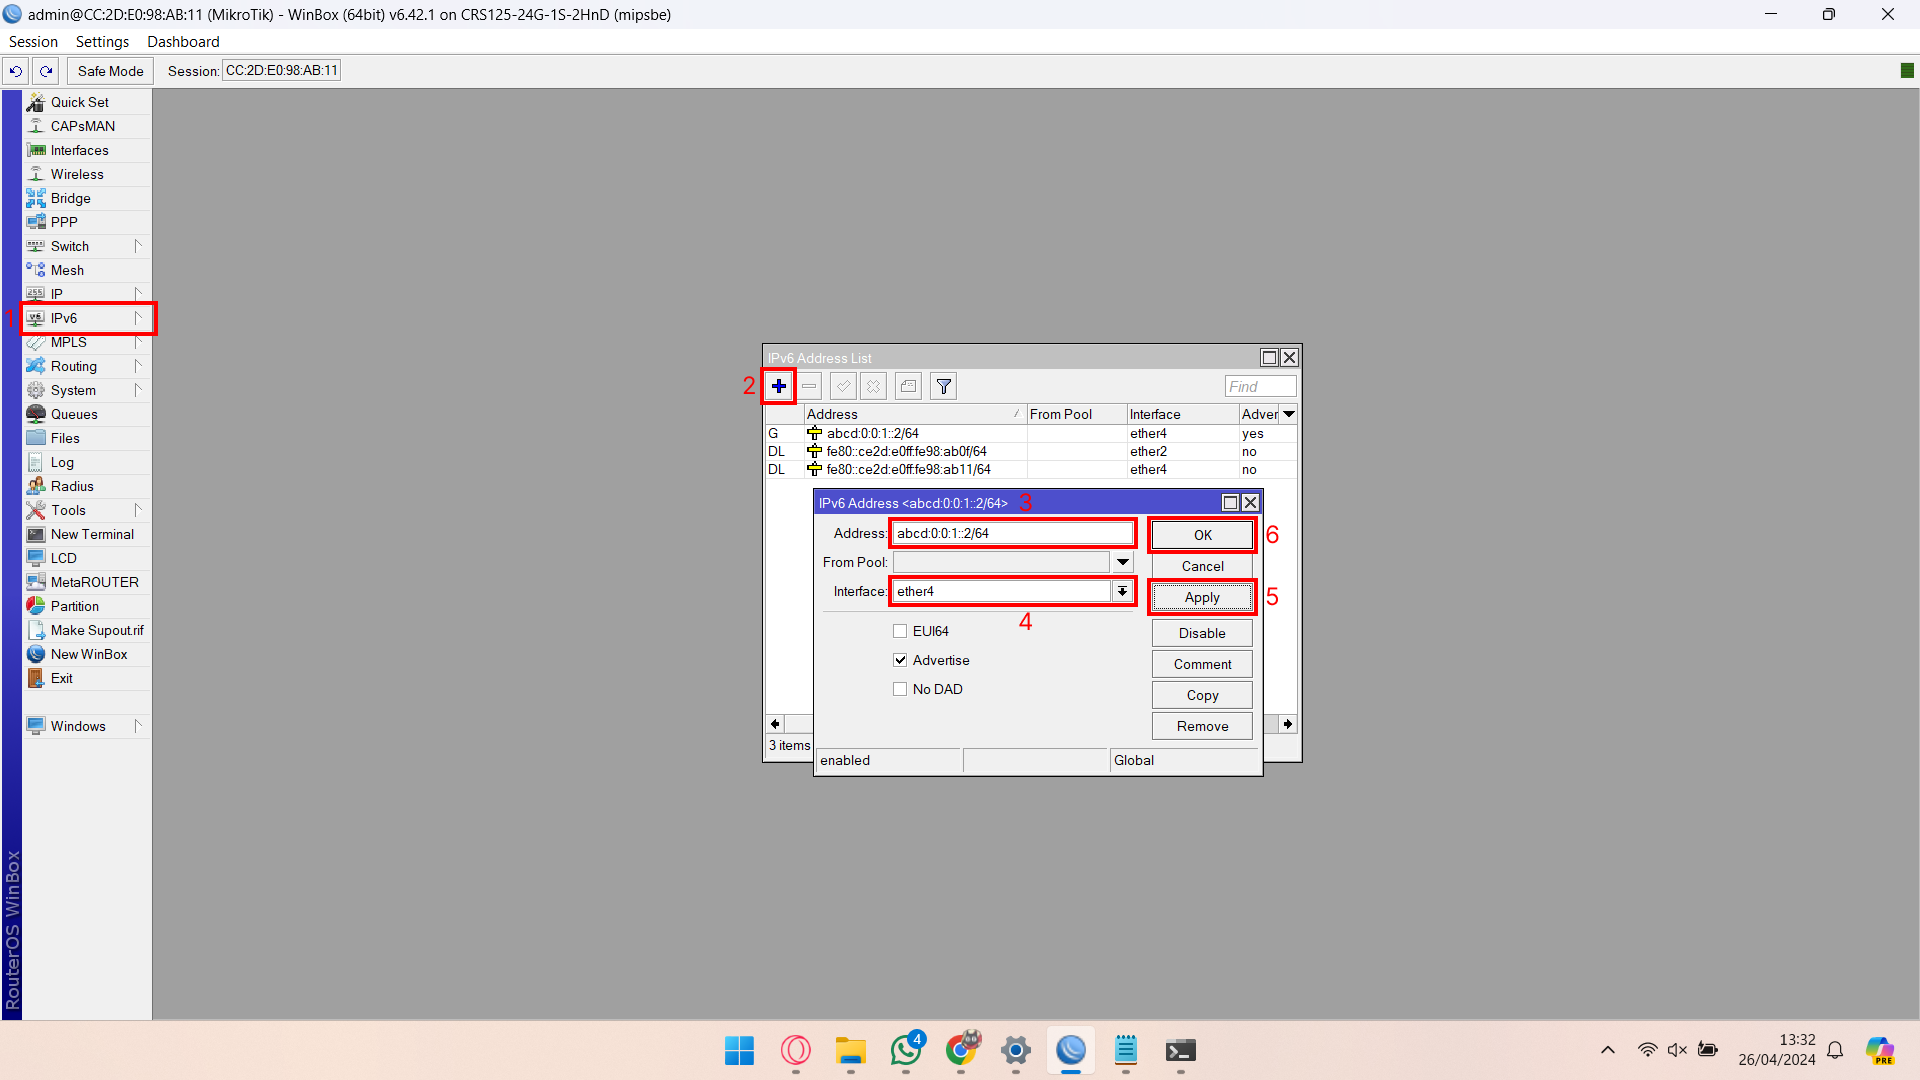
\includegraphics[width=0.8\linewidth]{P5/img/pc1/Step 3.png}
			\caption{Step 3}
			\label{fig:Step 3(PC 1)}
		\end{figure}

        \item Konfigurasi IPv6 pada PC 1 dengan mengubah pengaturan pada setting ethernet. Ubah IPv6 perangkat yang otomatis menjadi manual, pastikan IPv6 PC 1 masih satu jaringan dengan IPv6 lokal yang diinginkan, isi Gateway dengan IPv6 address Router 1 yang tersambung dengan PC 1. Berikan IPv6 address yang berbeda dengan contoh yang ada di modul.
        \begin{figure}[H]
			\centering
			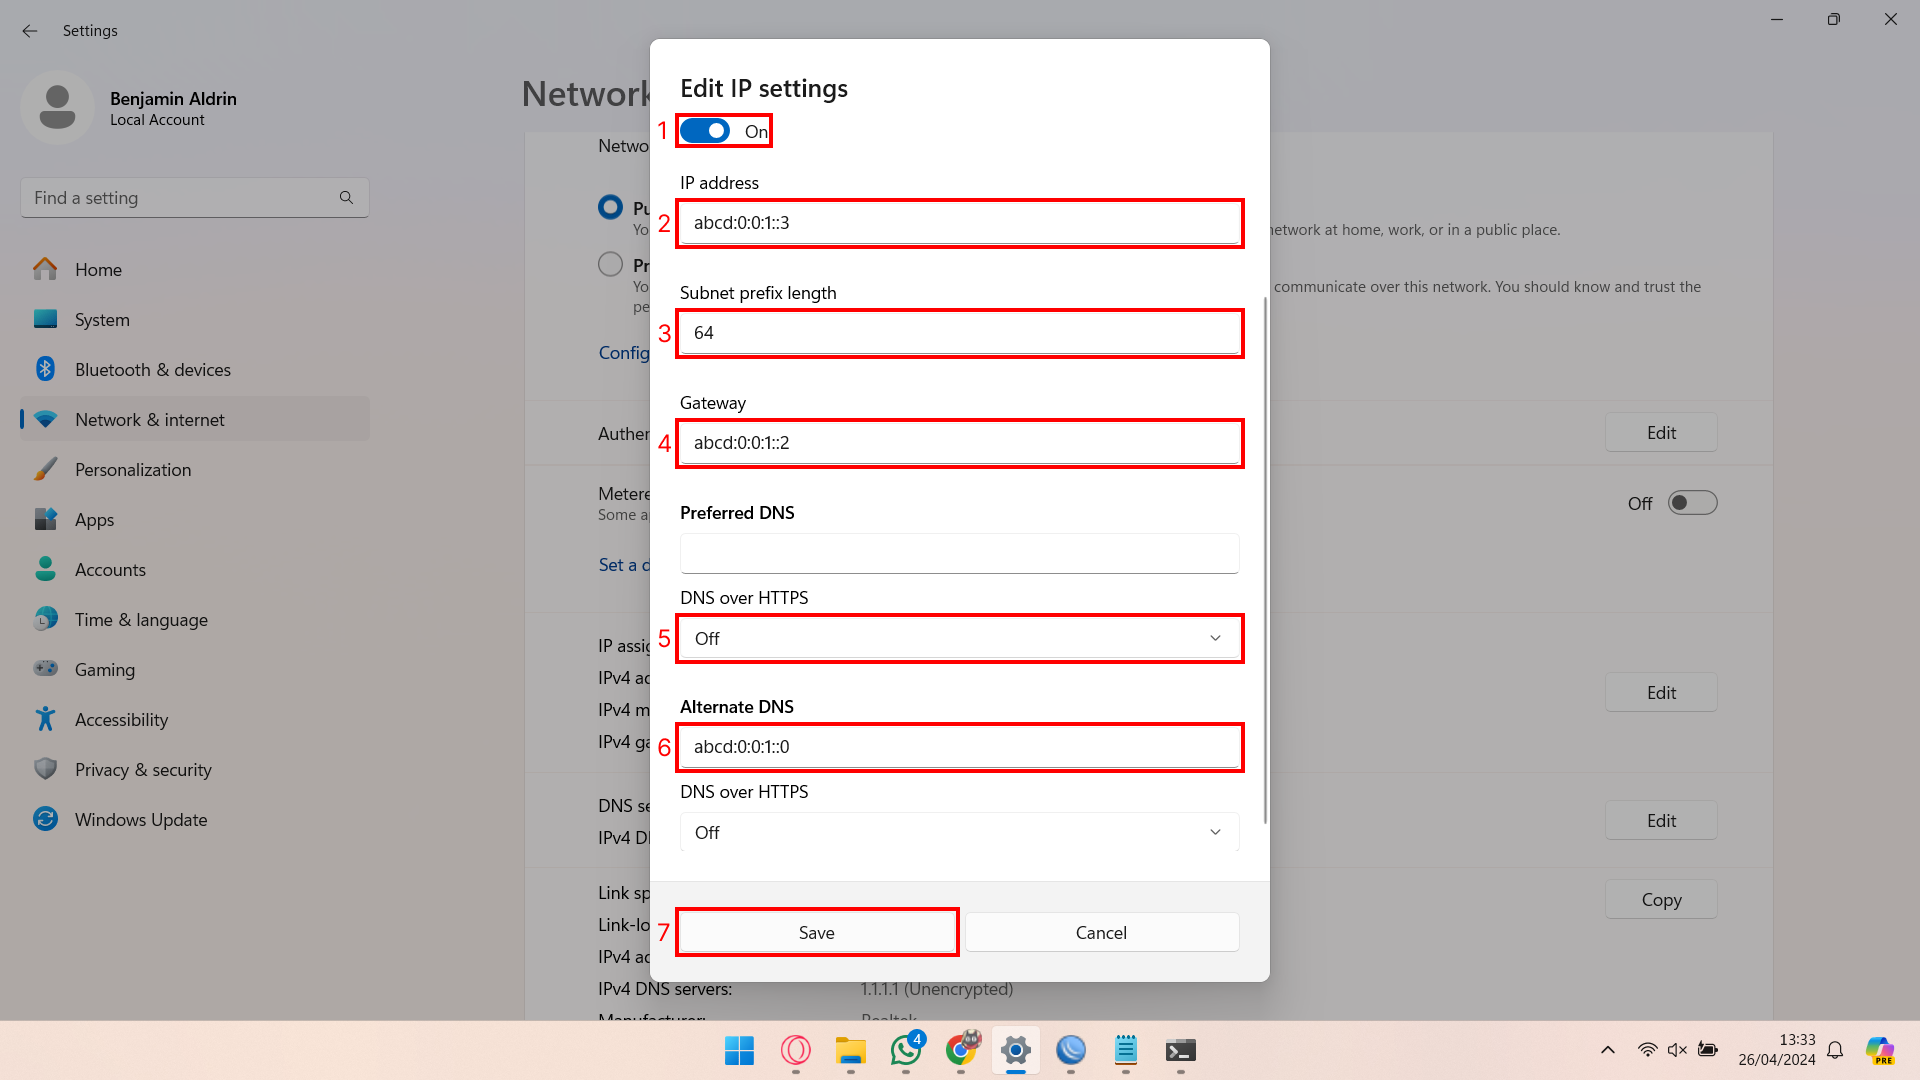
\includegraphics[width=0.8\linewidth]{P5/img/pc1/Step 4.png}
			\caption{Step 4}
			\label{fig:Step 4(PC 1)}
		\end{figure}

        \item Lakukan uji coba ping dari Router 1 ke PC 1 dan sebaliknya untuk memastikan kedua perangkat sudah saling terhubung.
        \begin{figure}[H]
			\centering
			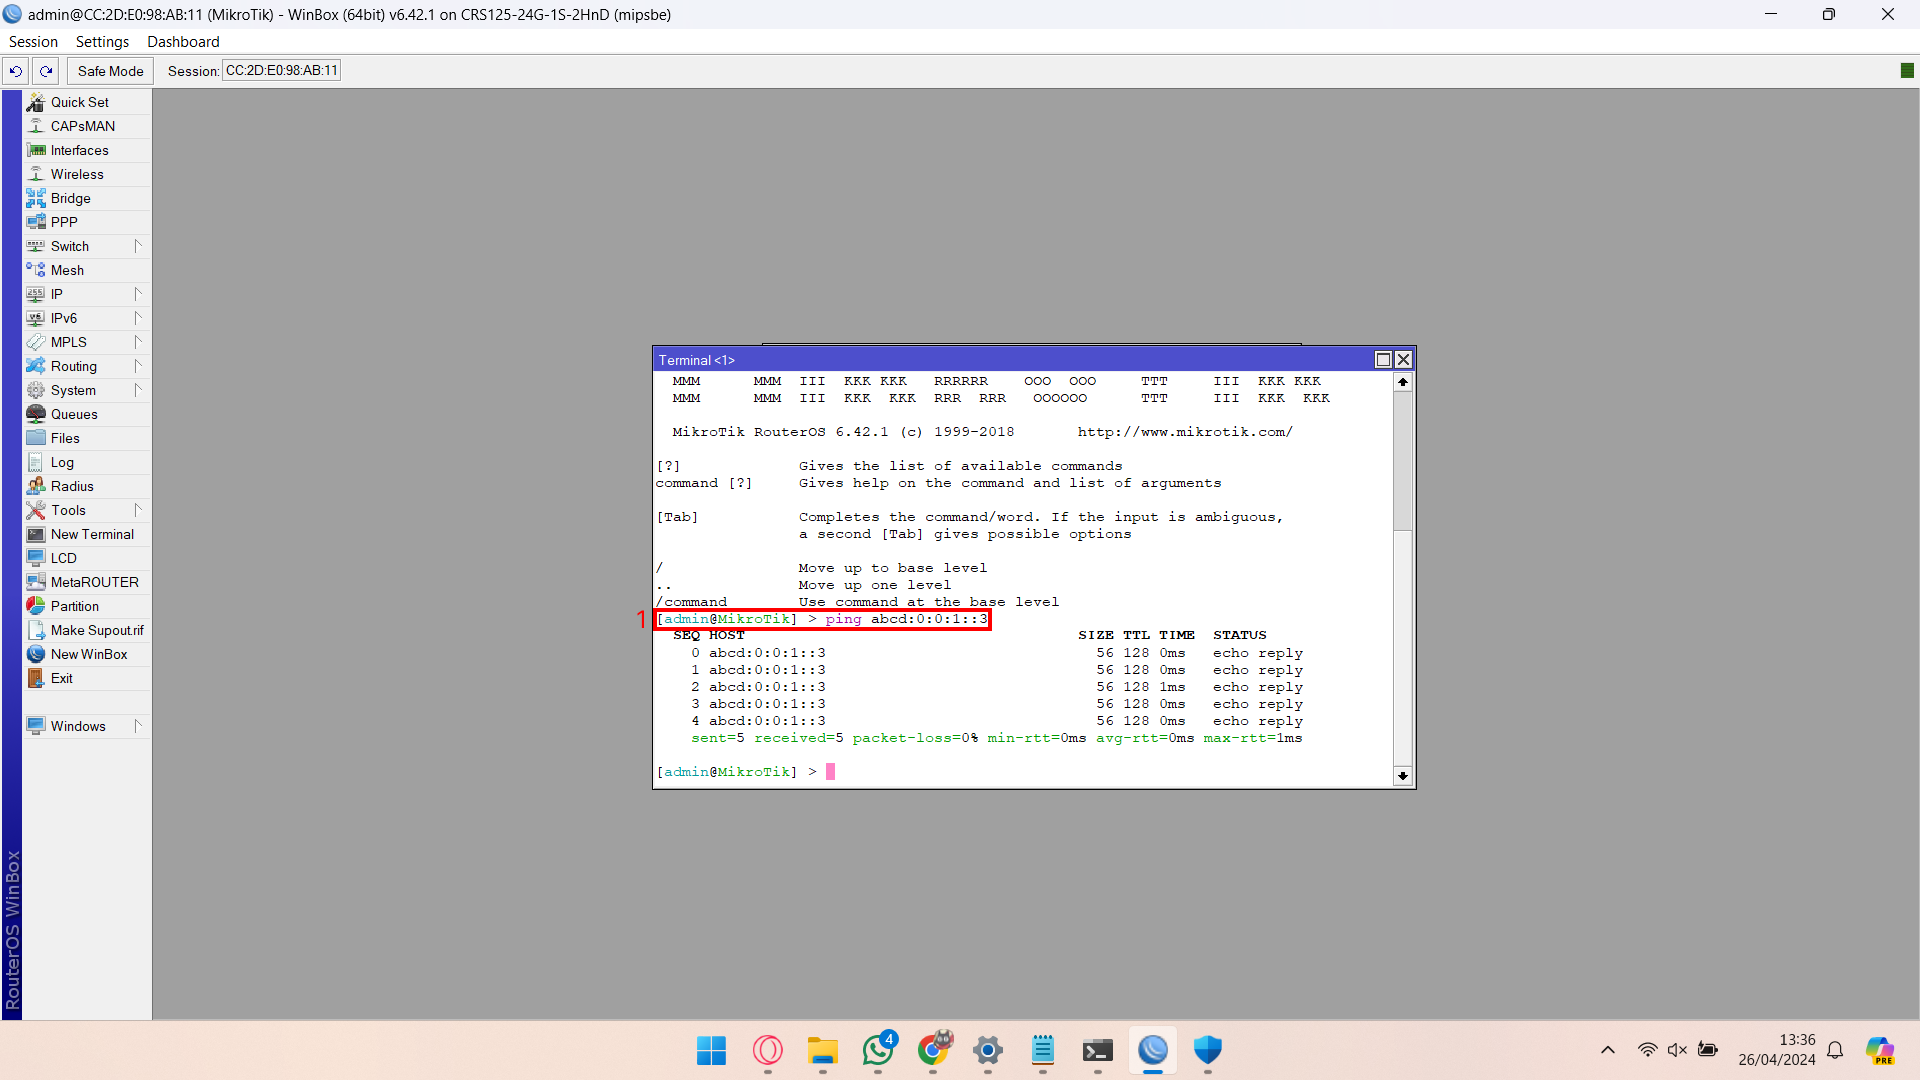
\includegraphics[width=0.8\linewidth]{P5/img/pc1/Step 5.png}
			\caption{Step 5}
			\label{fig:Step 5(PC 1)}
		\end{figure}

        \item Konfigurasi IPv6 Router 1 untuk menghubungkan Router 1 dengan Router 2. Tambahkan address IPv6 > Isi address > pilih Interface yang terhubung ke Router 2 (ether2) > Klik Apply > Klik OK.
        \begin{figure}[H]
			\centering
			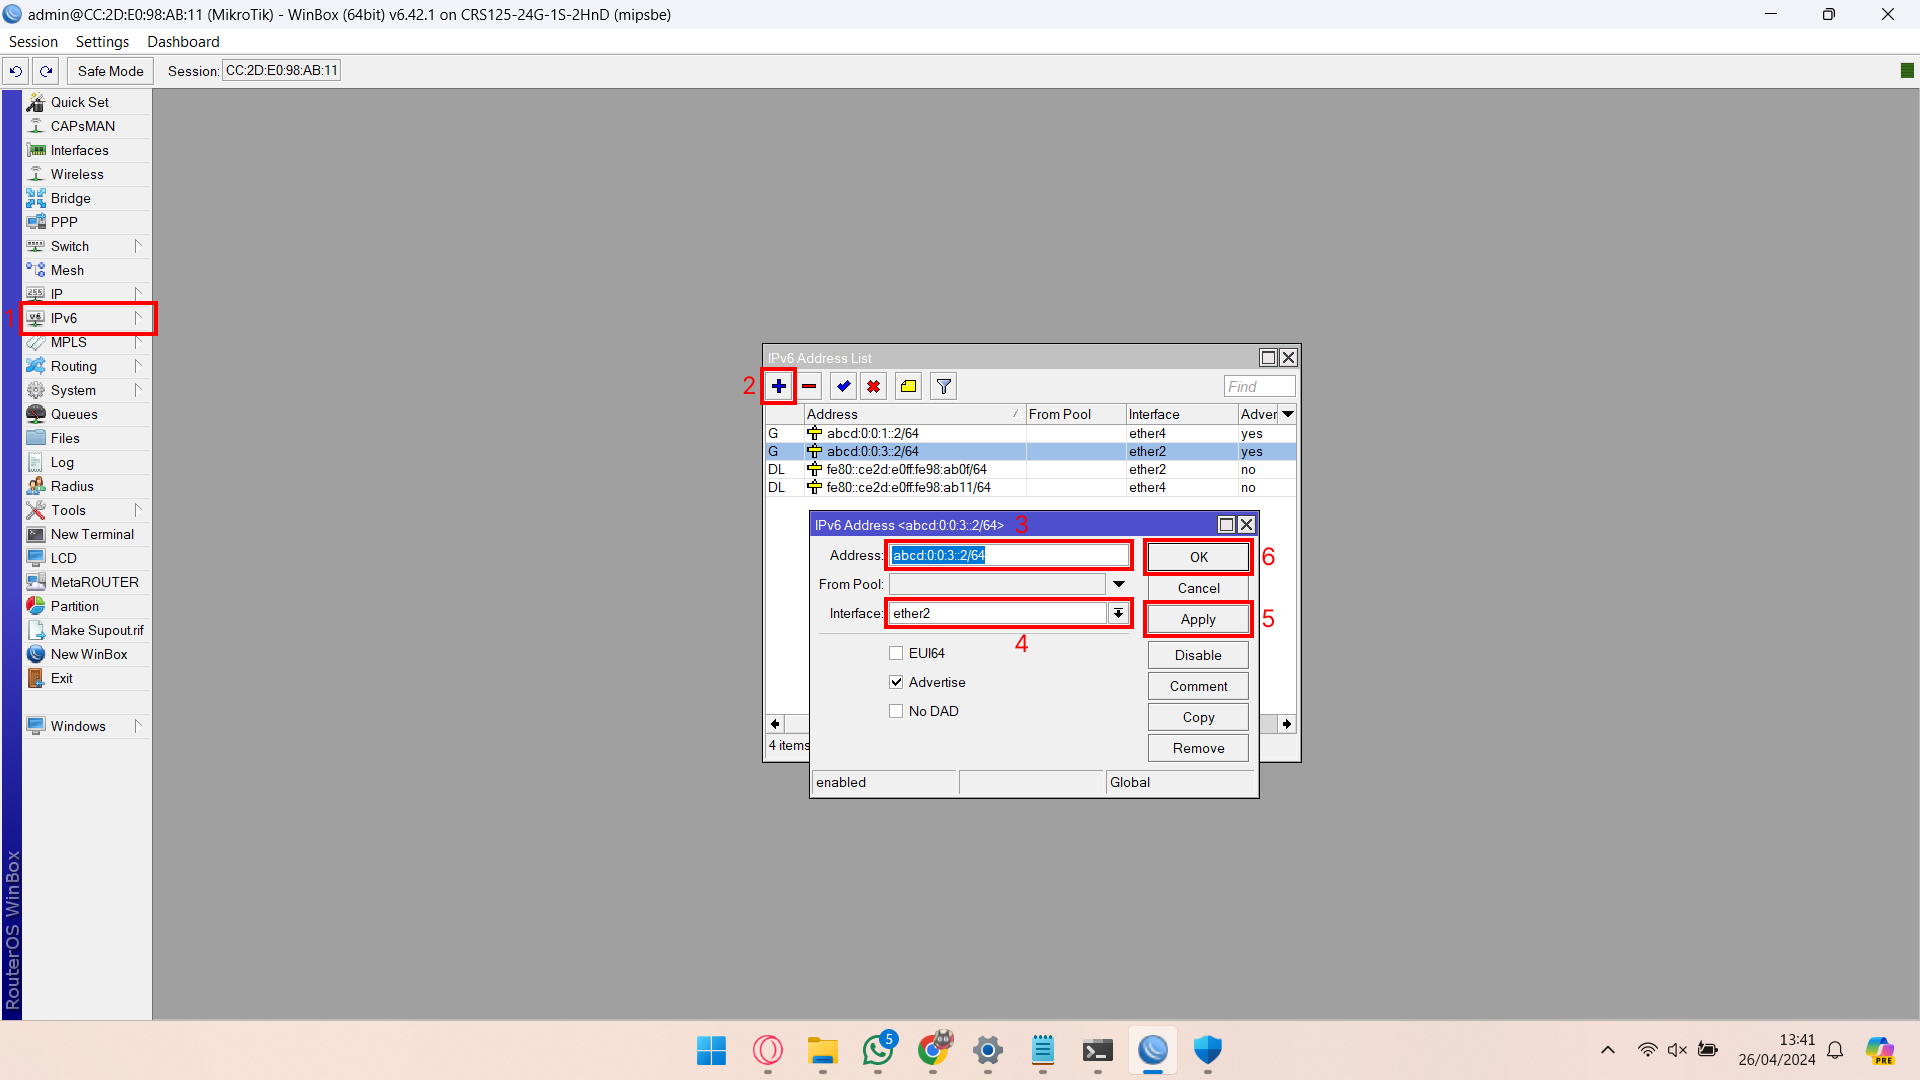
\includegraphics[width=0.8\linewidth]{P5/img/pc1/Step 6.png}
			\caption{Step 6}
			\label{fig:Step 6(PC 1)}
		\end{figure}

        \item Hubungkan kedua Network menggunakan routing statis. Buka pada tab IPv6 > Routes. Lalu tambahkan routes. Masukkan alamat jaringan yang ingin dituju, melalui alamat Gateway pada Router 2.
        \begin{figure}[H]
			\centering
			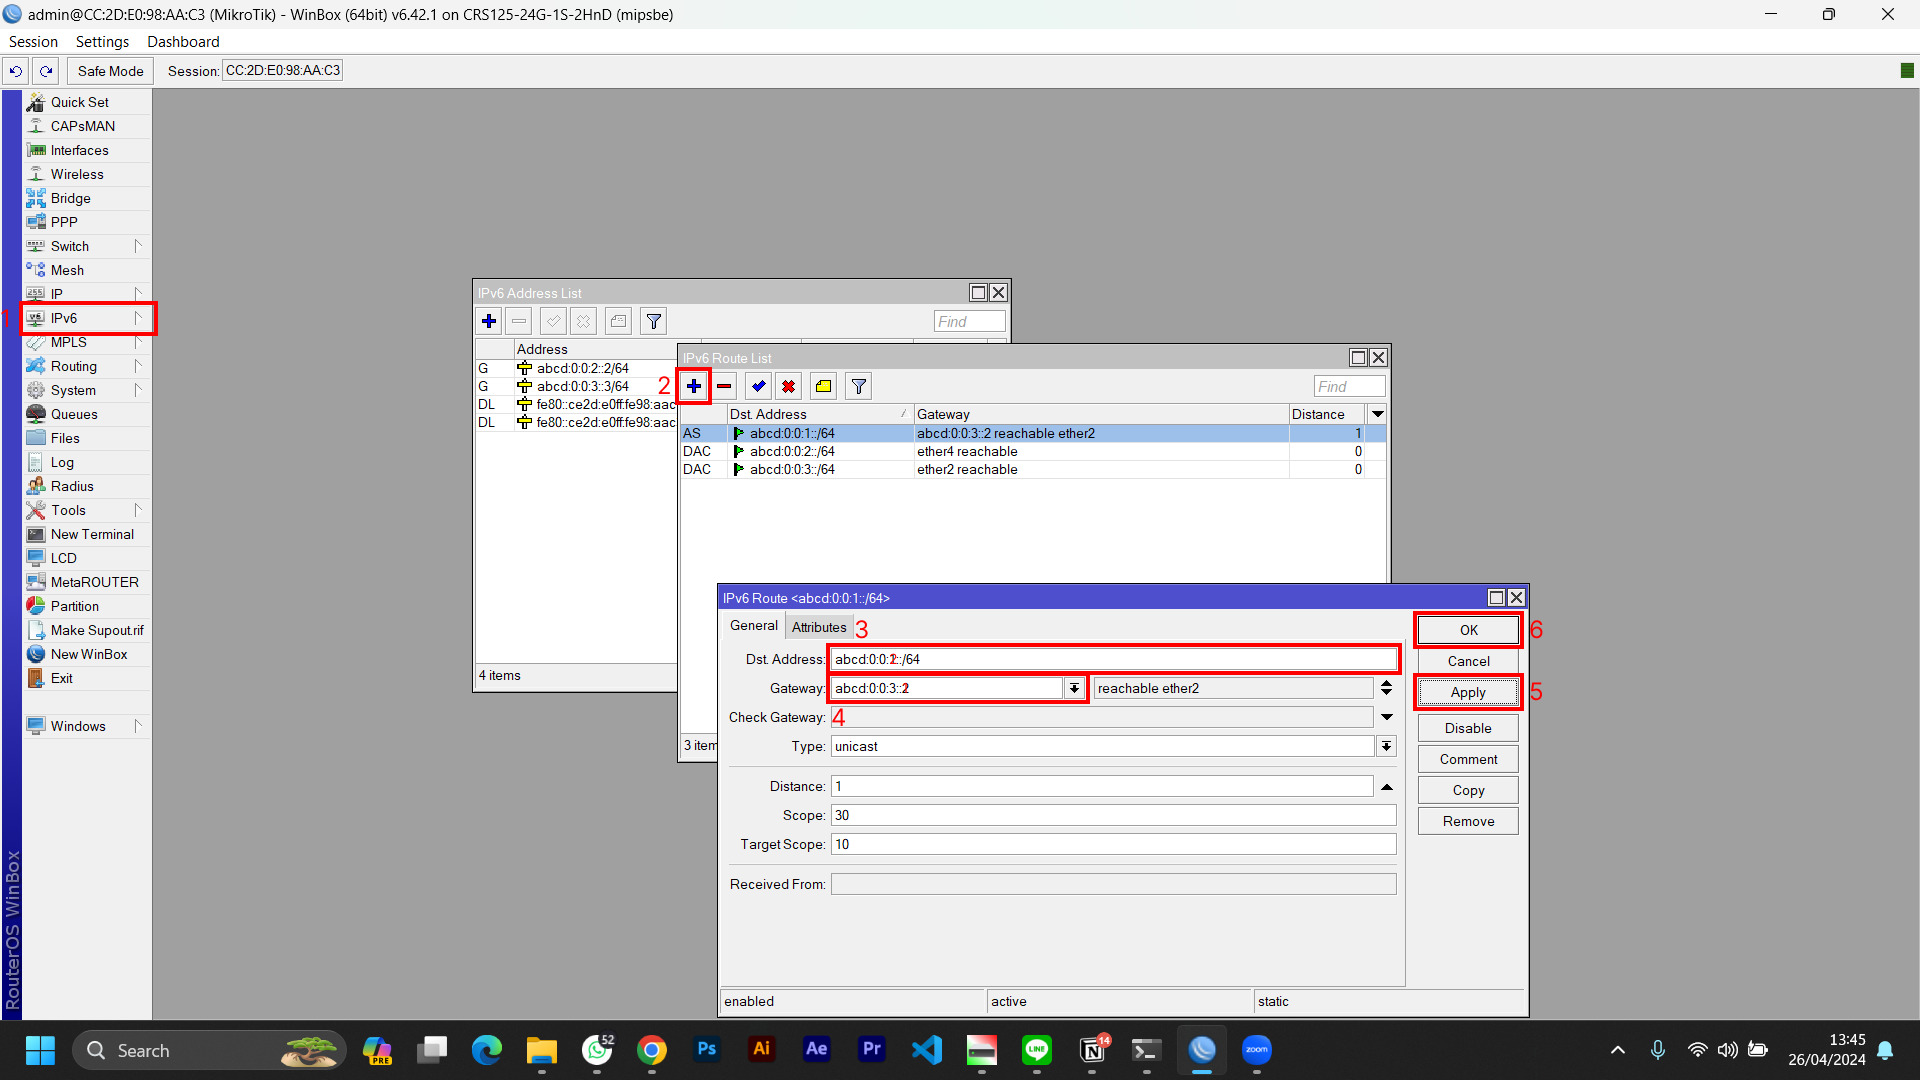
\includegraphics[width=0.8\linewidth]{P5/img/pc1/Step 7.png}
			\caption{Step 7}
			\label{fig:Step 7(PC 1)}
		\end{figure}
    \end{enumerate}

    \textbf{Konfigurasi PC 2}
    \begin{enumerate}
        \item Buka aplikasi Winbox pada PC2 dan hubungkan ke Router. Pastikan Login terisi “admin”, Klik Neighbors > Klik Refresh > Pilih Router yang ingin disambungkan > Klik Connect.
        \begin{figure}[H]
			\centering
			\includegraphics[width=0.5\linewidth]{P5/img/pc2/Step 1.png}
			\caption{Step 1}
			\label{fig:Step 1(PC 2)}
		\end{figure}
        \item Konfigurasikan Router2 untuk mengaktifkan layanan IPv6. Klik System > Klik Packages > Klik IPv6 > Klik Enable > Reboot ulang Router2.
        \begin{figure}[H]
			\centering
			\includegraphics[width=0.5\linewidth]{P5/img/pc2/Step 2.png}
			\caption{Step 2}
			\label{fig:Step 2(PC 2)}
        \end{figure}
        \item Konfigurasi IPv6 Router 2 untuk menghubungkan PC 2 dengan Router 2. Tambahkan IP address > Isi address > pilih Interface yang terhubung ke PC 2 (ether4) > Klik Apply > Klik OK.
        \begin{figure}[H]
			\centering
			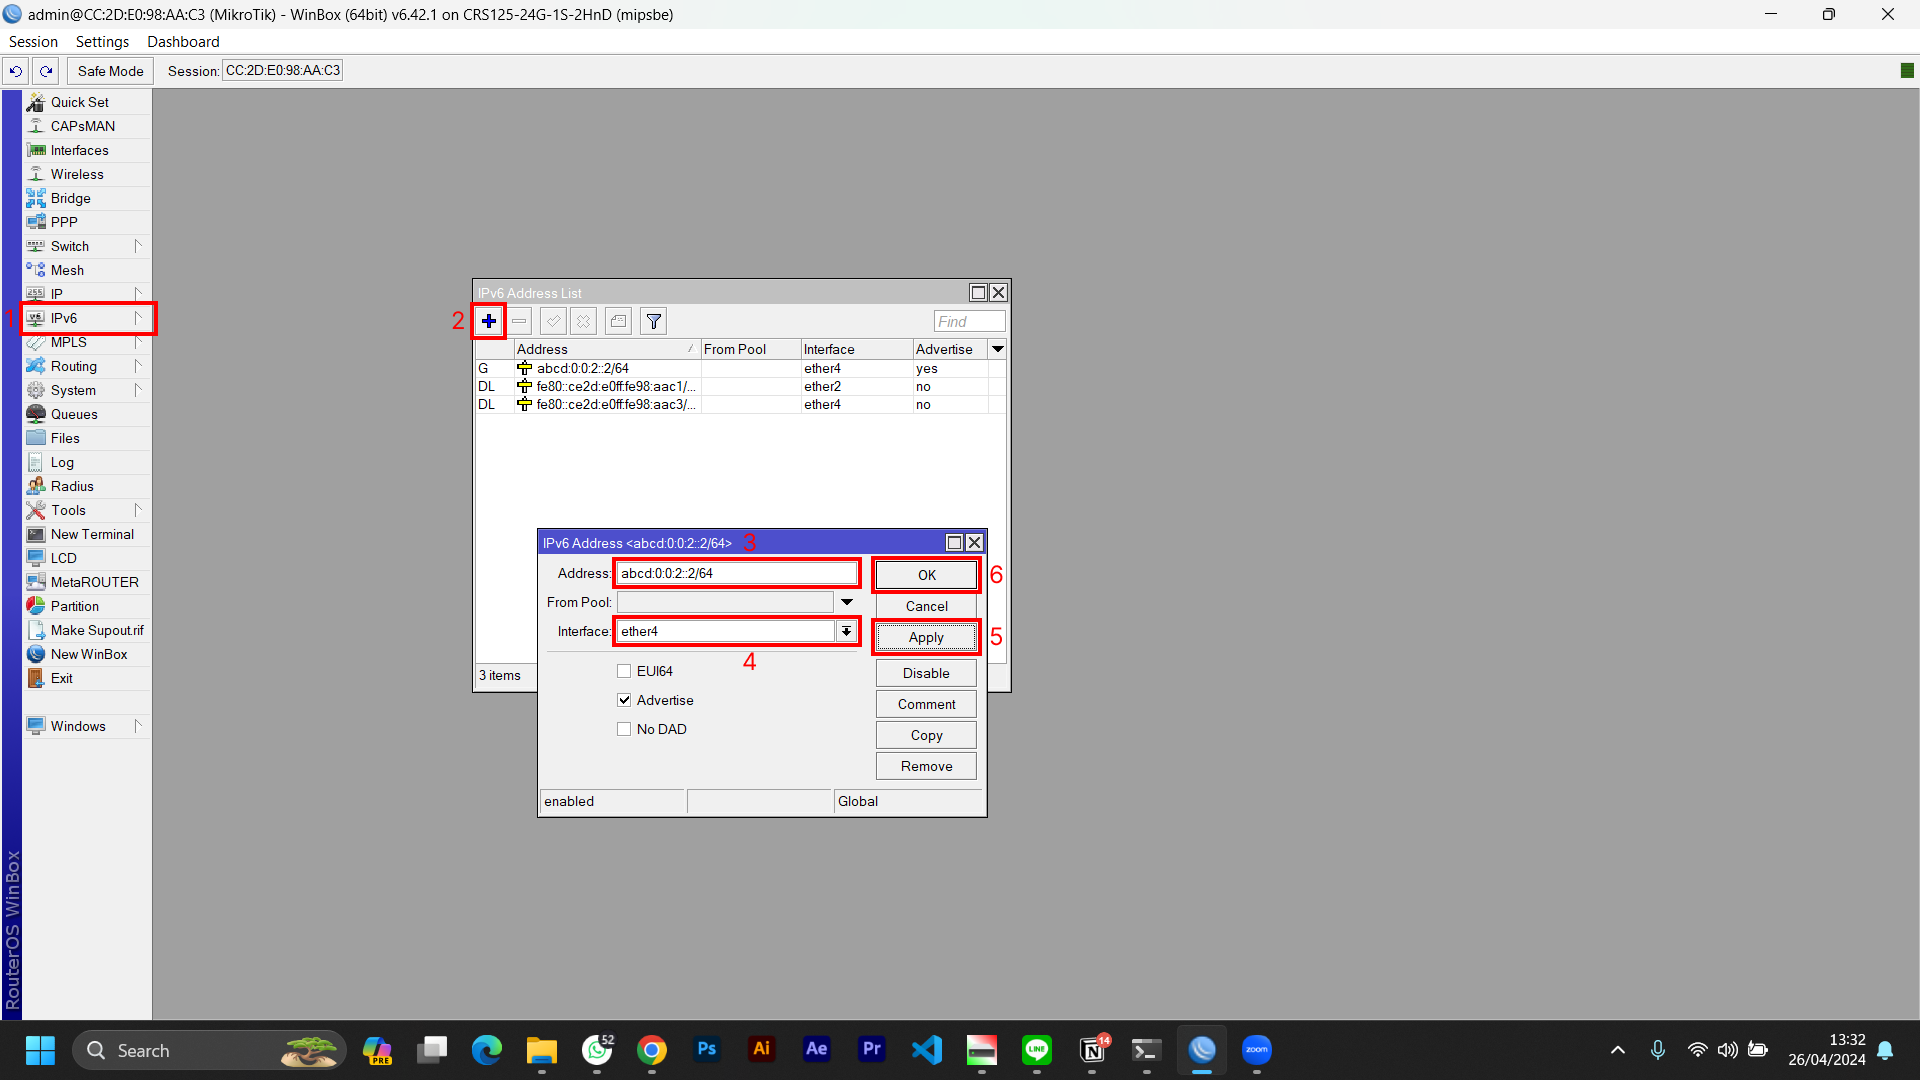
\includegraphics[width=0.8\linewidth]{P5/img/pc2/Step 3.png}
			\caption{Step 3}
			\label{fig:Step 3(PC 2)}
		\end{figure}
        \item Konfigurasi IPv6 pada PC 2 dengan mengubah pengaturan pada setting ethernet. Ubah IPv6 perangkat yang otomatis menjadi manual, pastikan IPv6 PC 2 masih satu jaringan dengan IPv6 lokal yang diinginkan, isi Gateway dengan IPv6 address Router 2 yang tersambung dengan PC 2. Berikan IPv6 address yang berbeda dengan contoh yang ada di modul.
        \begin{figure}[H]
			\centering
			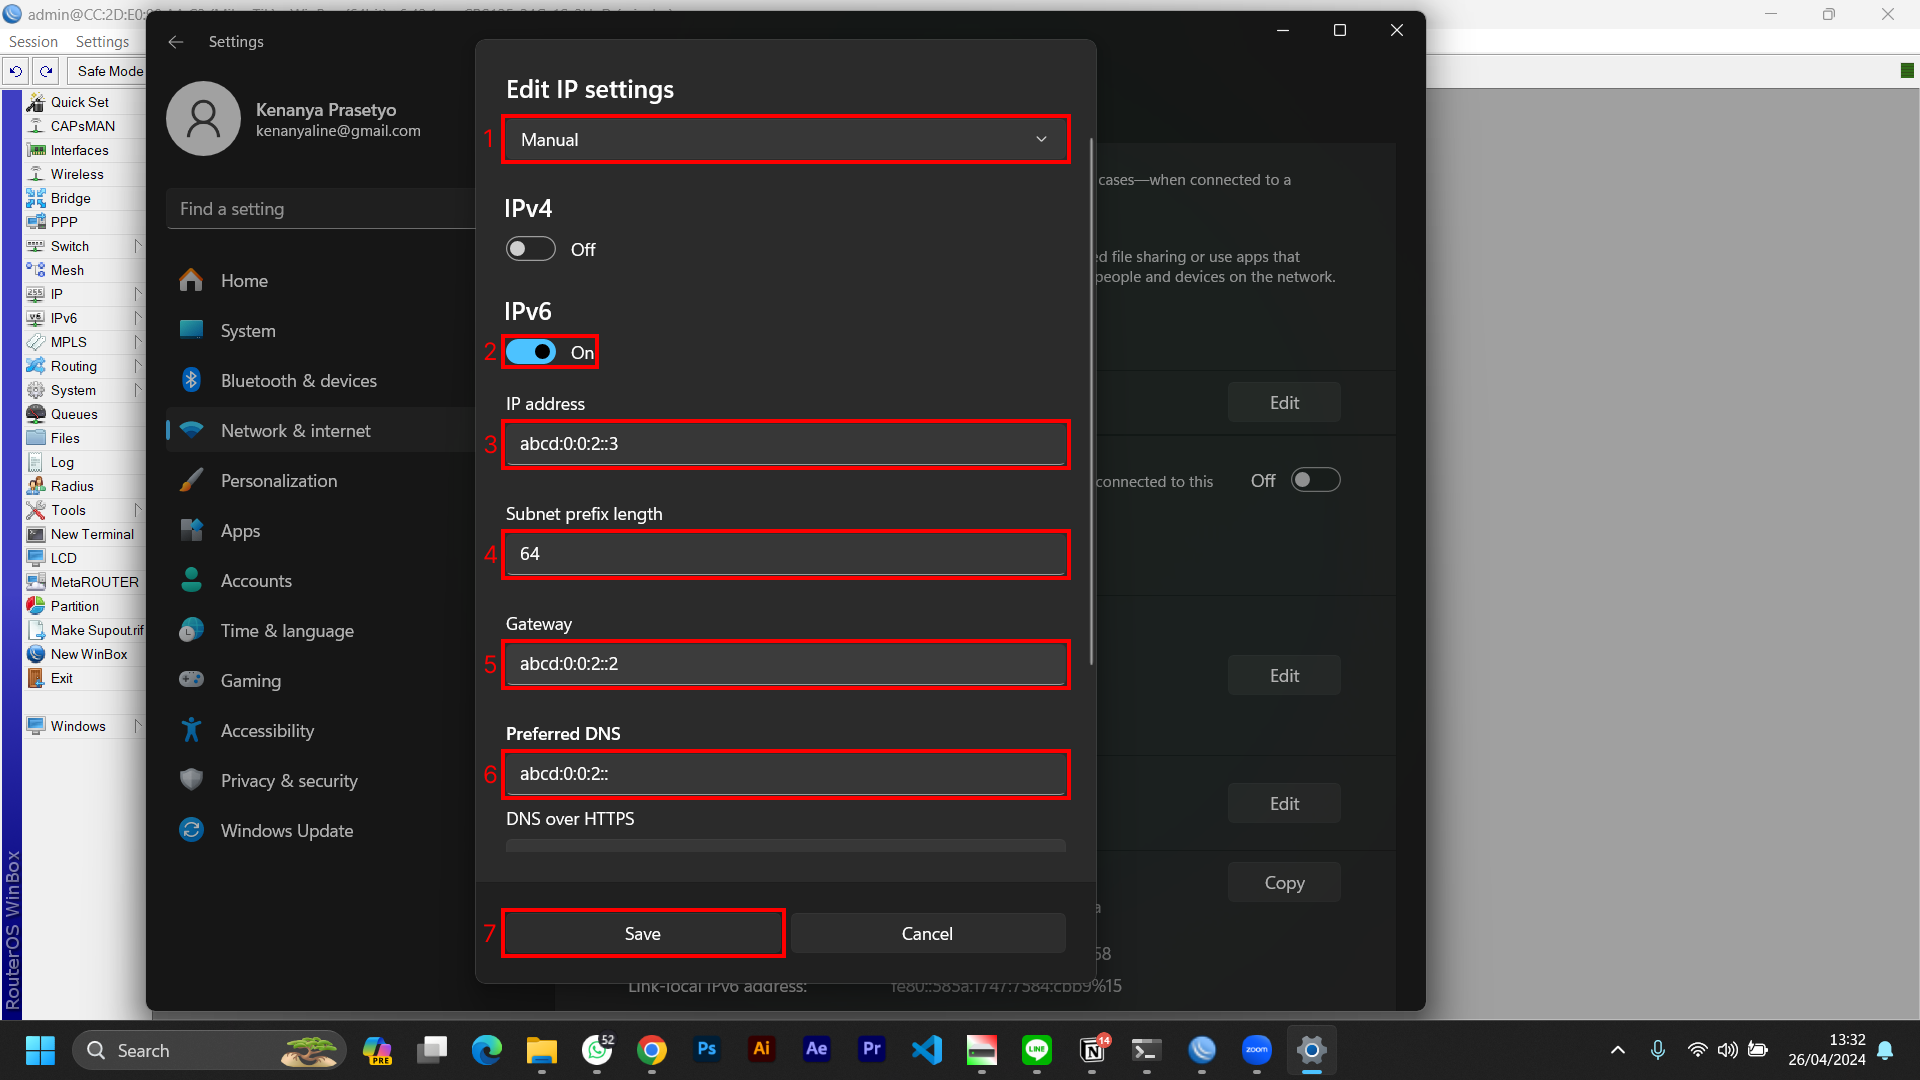
\includegraphics[width=0.8\linewidth]{P5/img/pc2/Step 4.png}
			\caption{Step 4}
			\label{fig:Step 4(PC 2)}
		\end{figure}
        \item Lakukan uji coba ping dari Router 2 ke PC 2 dan sebaliknya untuk memastikan kedua perangkat sudah saling terhubung.
        \begin{figure}[H]
			\centering
			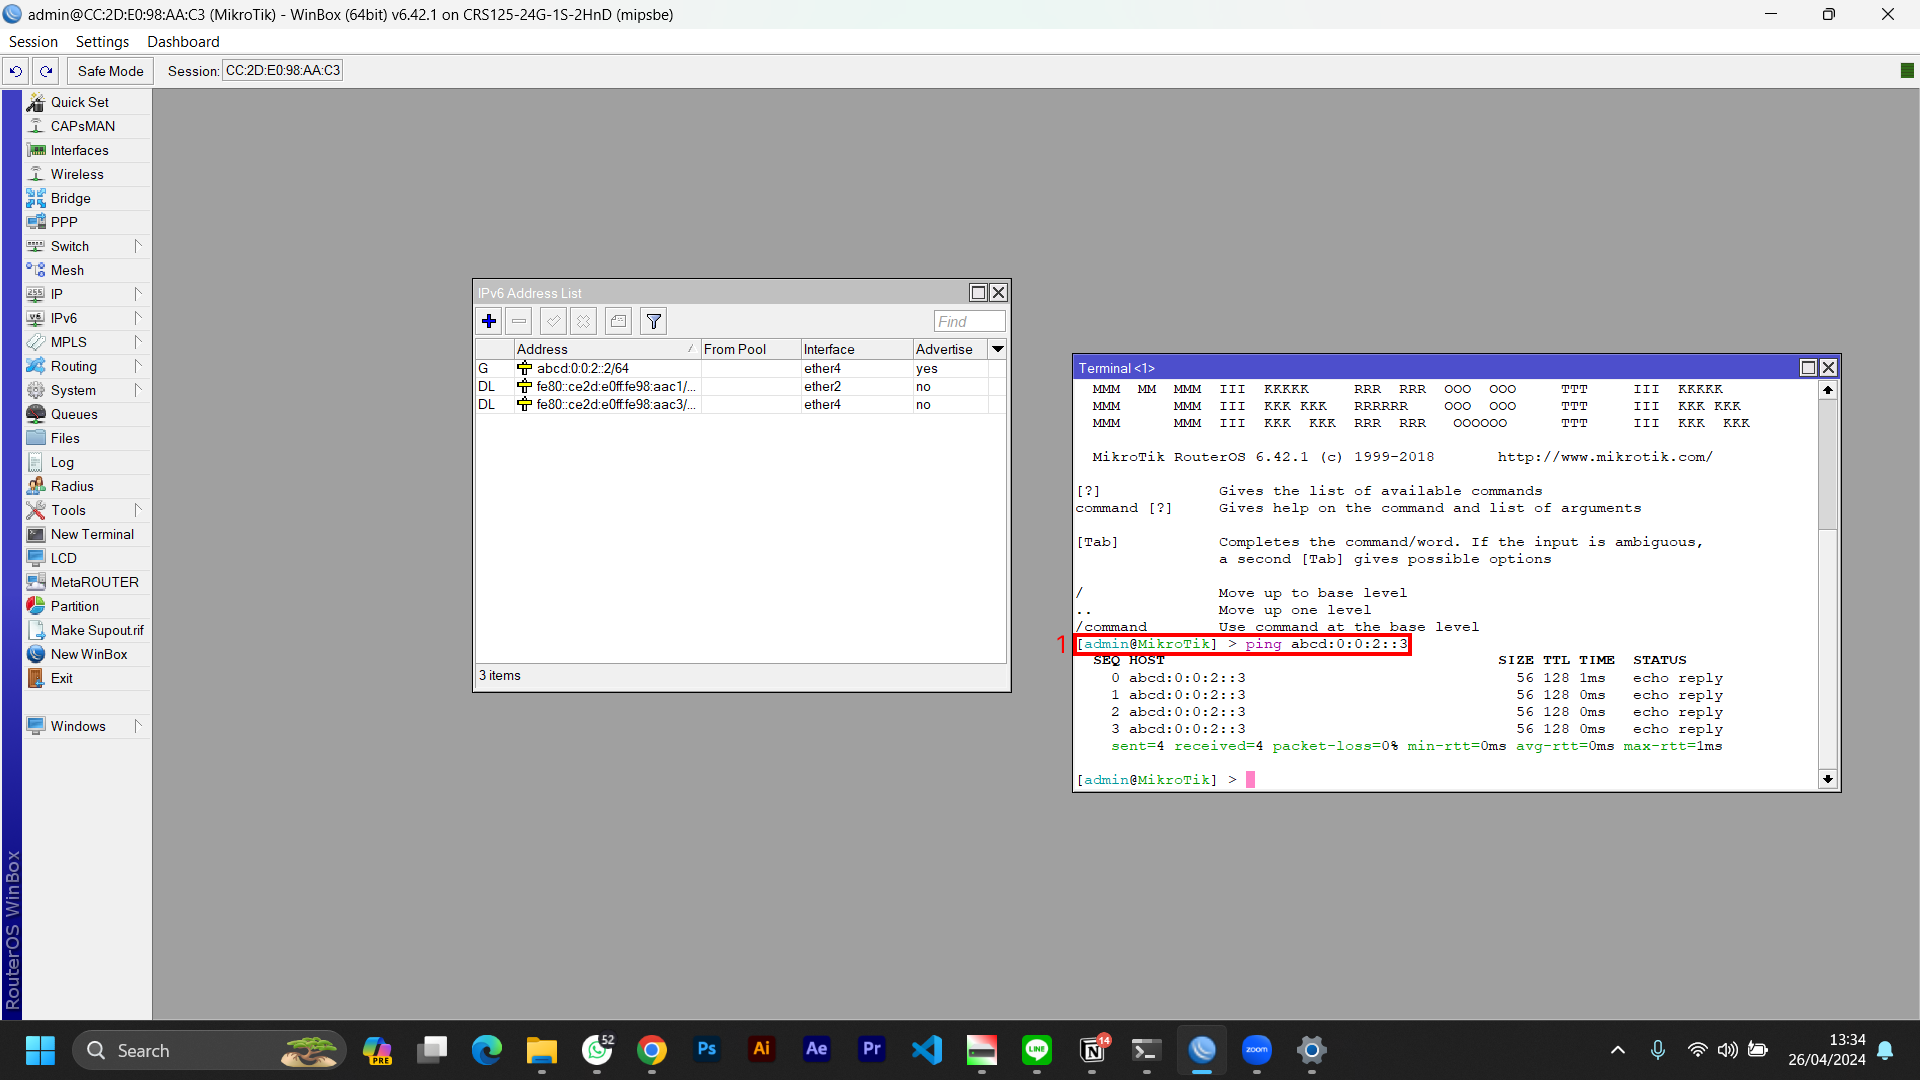
\includegraphics[width=0.8\linewidth]{P5/img/pc2/Step 5.png}
			\caption{Step 5}
			\label{fig:Step 5(PC 2)}
		\end{figure}
    
        \item Konfigurasi IPv6 Router 2 untuk menghubungkan Router 2 dengan Router 1. Tambahkan address IPv6 > Isi address > pilih Interface yang terhubung ke Router 1 (ether2) > Klik Apply > Klik OK.
        \begin{figure}[H]
			\centering
			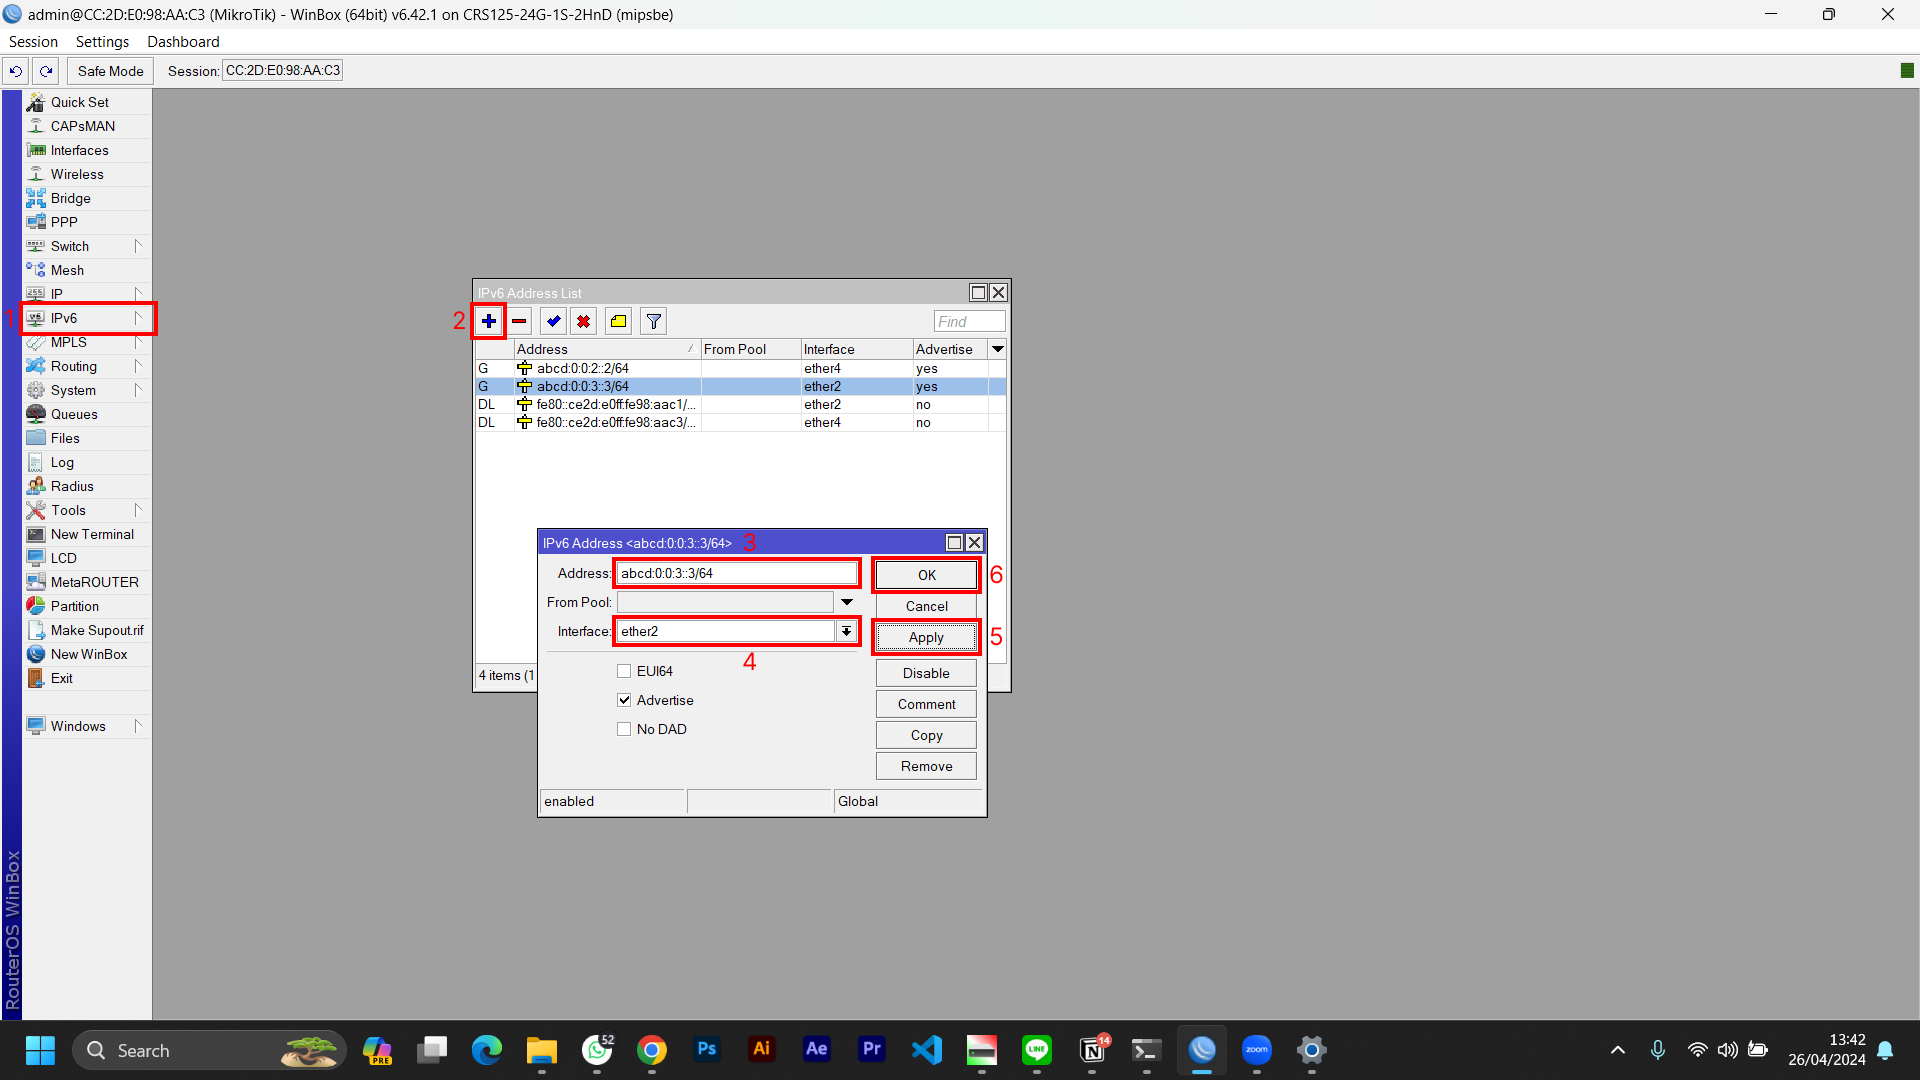
\includegraphics[width=0.8\linewidth]{P5/img/pc2/Step 6.png}
			\caption{Step 6}
			\label{fig:Step 6(PC 2)}
		\end{figure}
        \item Hubungkan kedua Network menggunakan routing statis. Buka pada tab IPv6 > Routes. Lalu tambahkan routes. Masukkan alamat jaringan yang ingin dituju, melalui alamat Gateway pada Router 1.
        \begin{figure}[H]
			\centering
			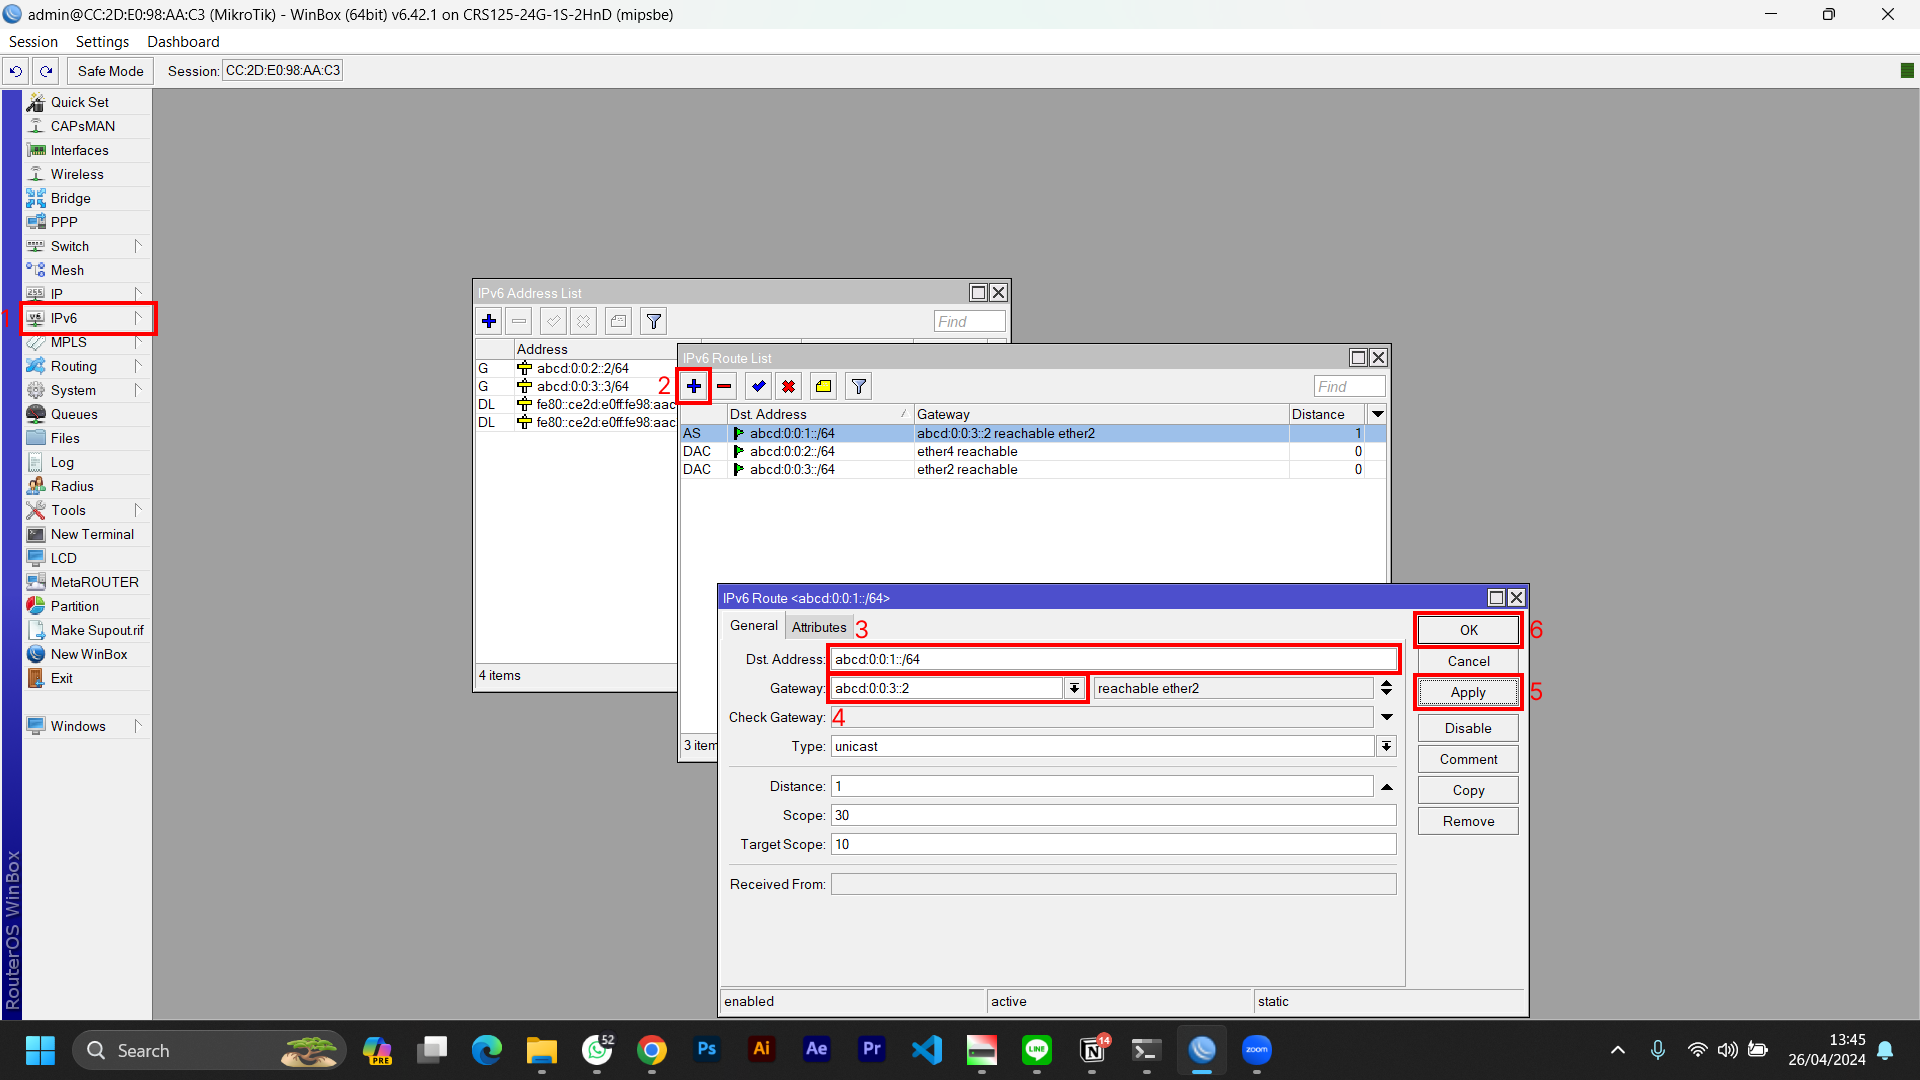
\includegraphics[width=0.8\linewidth]{P5/img/pc2/Step 7.png}
			\caption{Step 7}
			\label{fig:Step 7(PC 2)}
		\end{figure}
    \end{enumerate}

	\textbf{Pengujian Konfigurasi}
	\begin{enumerate}
		\item Lakukan tes ping ke alamat IPv6 PC 2 untuk memastikan kedua PC sudah terhubung.
		\begin{figure}[H]
			\centering
			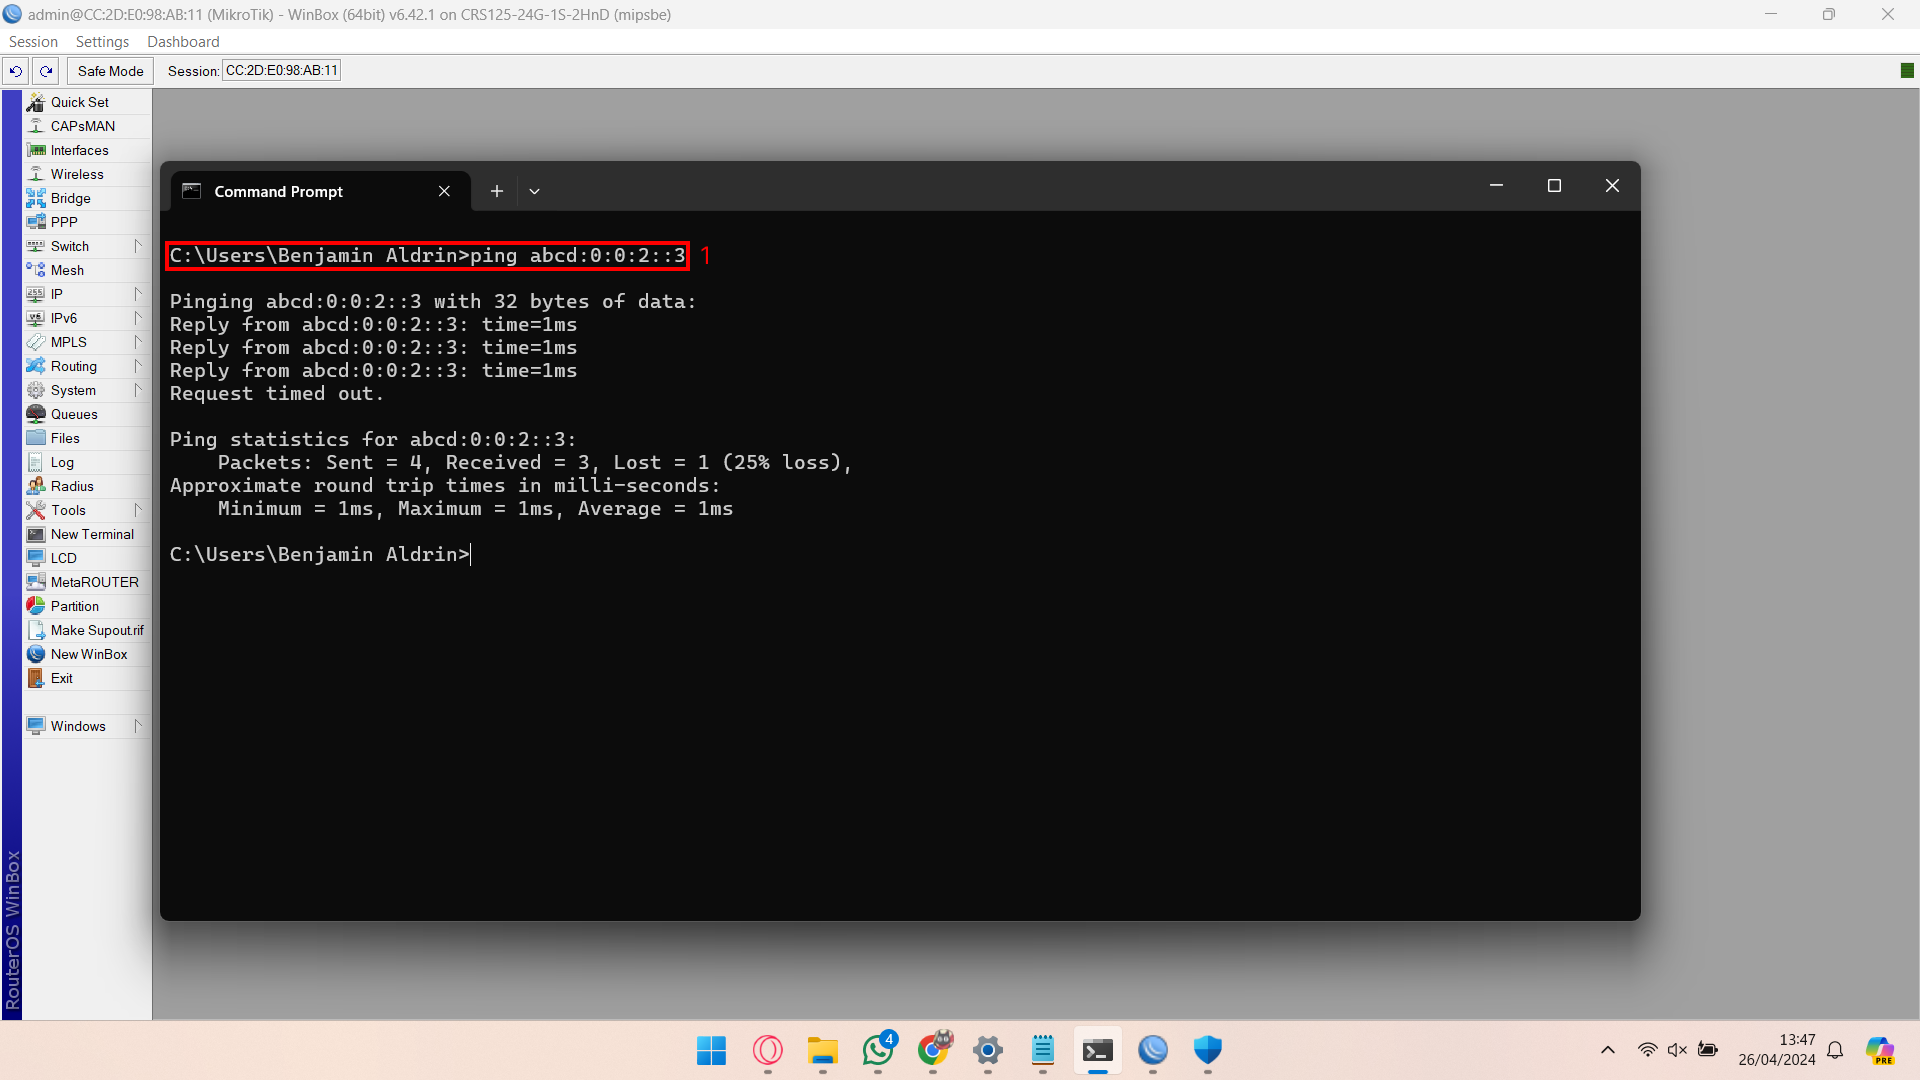
\includegraphics[width=0.8\linewidth]{P5/img/pc1/Step 8.png}
			\caption{Step 1}
			\label{fig:Ping Step 1}
		\end{figure}
        \item Lakukan tes ping ke alamat IPv6 PC 1 untuk memastikan kedua PC sudah terhubung.
		\begin{figure}[H]
			\centering
			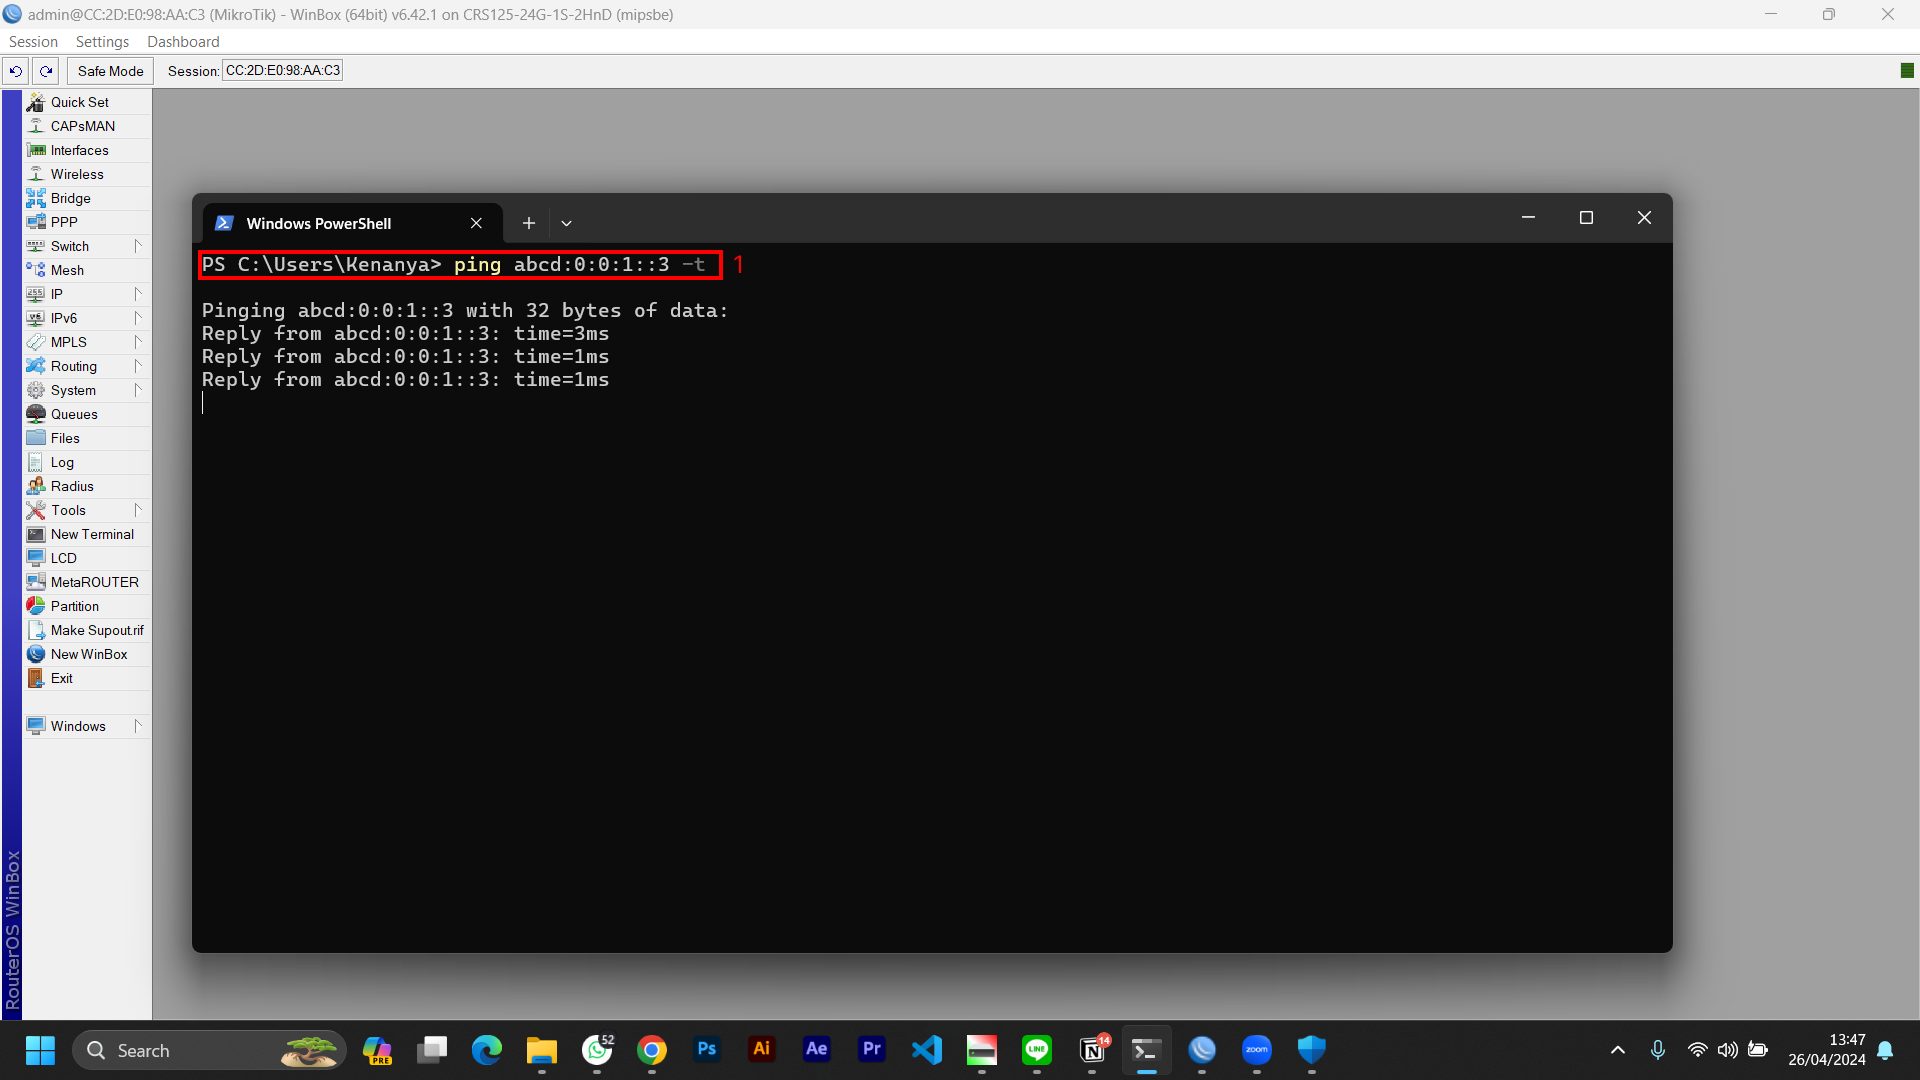
\includegraphics[width=0.8\linewidth]{P5/img/pc2/Step 8.png}
			\caption{Step 2}
			\label{fig:Ping Step 2}
		\end{figure}
	\end{enumerate}

\end{center}

%===========================================================%
\section{Hasil yang didapat}
Memahami penerapan dan penghubungan jaringan dengan menerapkan IPv6 pada konfigurasi statis

%===========================================================%
\section{Kesimpulan}
Dalam mengkonfigurasi IPv6, diperlukan pemahaman dasar mengenai penghubungan jaringan dengan menggunakan konfigurasi statis
